% arara: lualatex: { interaction: nonstopmode, synctex: no }
% arara: lualatex: { interaction: nonstopmode, synctex: no }
\documentclass[a4paper,12pt,chapterprefix=false,bibliography=totoc,listof=totoc,book]{scrreprt}

\usepackage{latex-style}

\lstdefinelanguage{Gherkin}{
    morekeywords = {
        Given,
        When,
        Then,
        And,
        Scenario,
        Feature,
        But,
        Background,
        Scenario Outline,
        Examples
    },
    sensitive=true,
    morecomment=[l]{\#},
    morestring=[b]",
    morestring=[b]',
    keywordstyle=\normalsize\bfseries\color{green},
    basicstyle=\small\ttfamily,
}

\setlength{\parindent}{0pt}
\newabbreviation{na}{N/A}{Not applicable}

\begin{document}
    \begin{flushright}
        GameBase
        \\
        Use-Case Specification: Login User
% \\
% For <Subsystem or Feature>
        \bigbreak
        Version 1.0
    \end{flushright}

    \tableofcontents

    \chapter{Use-Case: Login User}

    \section{Brief Description}
    The use case describes the login process for an existing user.

    \chapter{Flow of Events}
    \begin{figure}[H]
        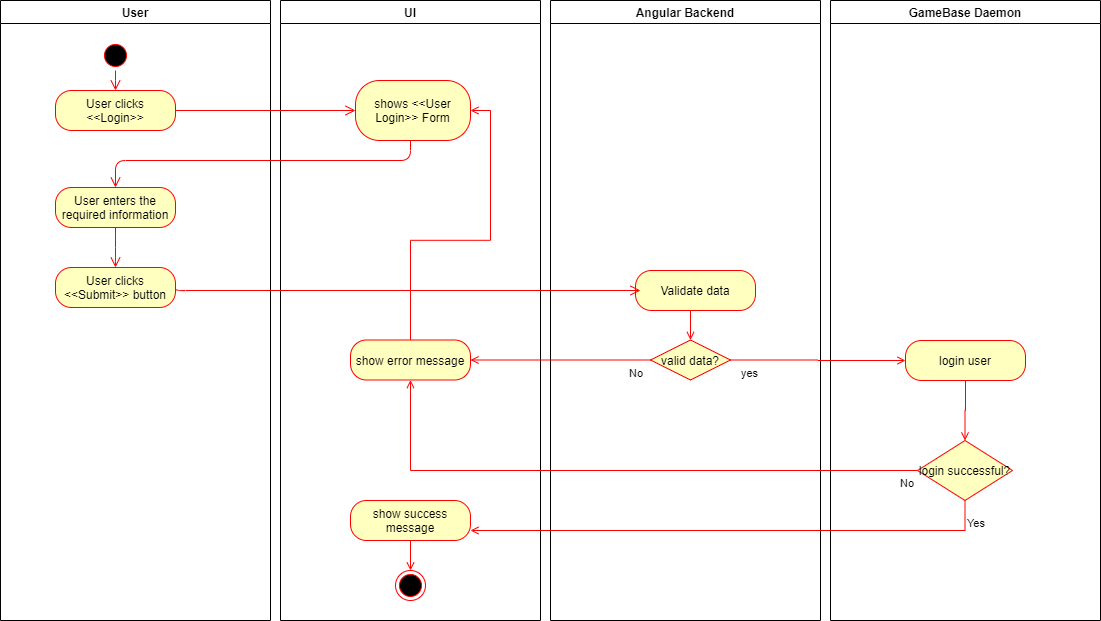
\includegraphics[width=\textwidth]{diagramms/UCLoginUserDiagramm.png}
        \caption{Activity Diagramm}
        \label{fig:ucd}
    \end{figure}
    \section{Basic flow}

    \begin{itemize}
        \item User clicks on <<Login>>
        \item User fills the form with the required information
        \item User clicks on <<Submit>> to log in
        \begin{itemize}
            \item On valid input: User redirected to overview page
            \item Otherwise: User is shown an error message
        \end{itemize}
    \end{itemize}


    \section{.feature File}
    \gls{na}

    \section{Imagery}
    \begin{figure}[H]
        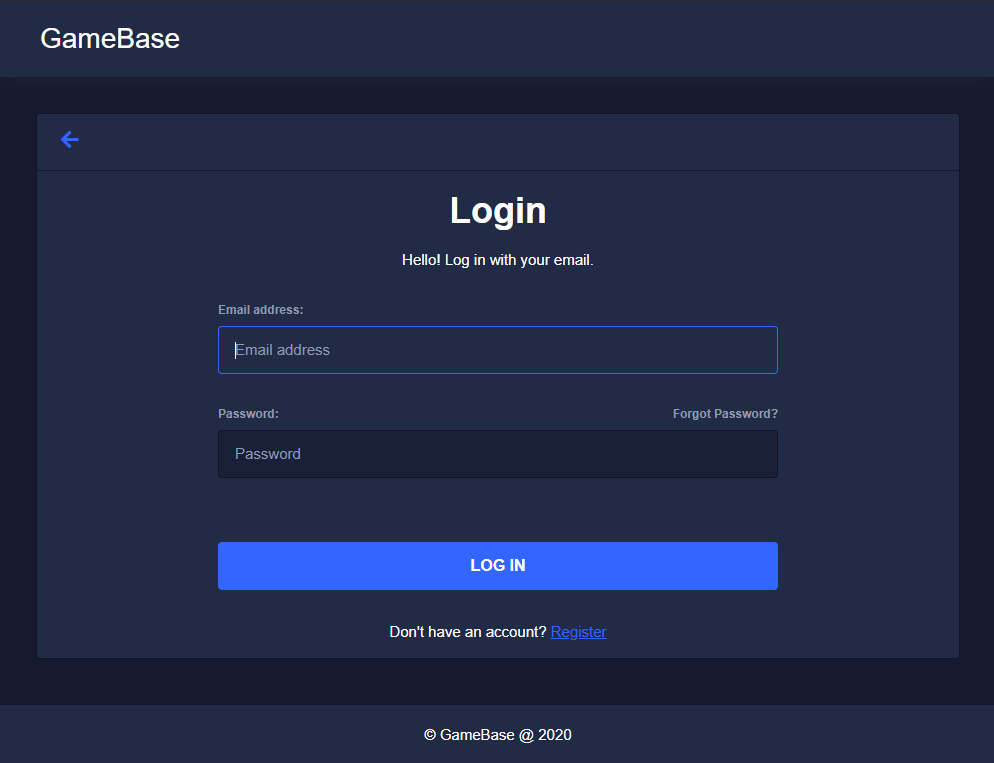
\includegraphics[width=\textwidth]{diagramms/UCLoginUserScreenshot.png}
        \caption{Activity Screenshot}
        \label{fig:screen}
    \end{figure}

    \chapter{Special Requirements}
    \section{Owning an account}
    The user has to be a registered user for our system.

    \chapter{Preconditions}
    \section{Is not logged in}
    The user must not be logged in.

    \chapter{Postconditions}
    \section{Is logged in}
    The user must be logged in and should be able to perform operations which require this condition.
\end{document}
